% El comienzo de esta rama de estudio de las matemáticas surge en el siglo XVII, motivado por problemas de geometría como el siguiente:

En Grecia se estudiaban problemas como el siguiente: si tengo una rueda con un punto en el borde y giro la rueda sobre una superficie plana resultará en la curva epicicloide. Sin embargo, esta solución se describía heurísticamente. Es por esto que tal y como la vamos a estudiar, el estudio de curvas y superficies surge en el siglo XVII con los dos autores más importantes de este siglo (y litigadores) Leibniz y Newton. En el siglo XVIII podemos estudiar a Euler y Monge. En el siglo XIX tenemos a Jean Frenet, Pauino Senet y autores de la Escuela Francesa, de entre ellos el más conocido, Cauchy. Por último del siglo XX tenemos a Jean Gaston Darboux y a Élie Cartan.

\chapter{Curvas en el plano y en el espacio}

\section{Definición. Curva Regular. Longitud de arco}

\begin{definicion}[Curva]
    Una \textbf{curva} en el espacio es una aplicación $\alpha: I \to \bb{R}^3$ diferenciable, donde $I\subseteq\bb{R}$ es un intervalo abierto. Normalmente, si queremos señalar las componentes de $\alpha$ escribiremos
    \begin{gather*}
        \alpha(t) = (x(t), y(t), z(t))
    \end{gather*}
    En realidad a un geómetra solo le interesa la llamada \textbf{traza de la curva}, definida como
    \begin{gather*}
        tr (\alpha) = img (\alpha) = \alpha(I)
    \end{gather*}
\end{definicion}

\begin{ejemplo}
    Sea $a\in \bb{R}^3$ un punto y $v\in \bb{R}^3$ un vector\footnote{Lo de llamar punto o vector solo sirve para facilitar el lenguaje y nuestro aprendizaje}. Definimos 
    \Func{\alpha}{\bb{R}}{\bb{R}^3}{t}{a+tv}
    Si estudiamos la traza de $\alpha$ veremos que tenemos que hacer una distinción de casos:

    \begin{itemize}
        \item Si $v=0$ tendremos que $img(\alpha) = \{a\}$ por lo que será un único punto y según nuestra definición esta será una recta.
        \item Si $v\neq 0$ tendremos ahora que $tr(\alpha)$ es la recta que pasa por $a$ y que tiene como vector de dirección el vector $v$, que escribiremos como 
        \begin{gather*}
            R_{a,v} = a + \langle v \rangle
        \end{gather*}
    \end{itemize}
\end{ejemplo}

\begin{definicion}[Curva plana]
    Una curva $\alpha: I \to \bb{R}^3$ la llamaremos \textbf{curva plana} si existe un plano $P\subset \bb{R}^3$ tal que $tr(\alpha)\subset P$.

    Como $P$ y $P(\{z=0\})$ son equivalentes por un movimiento rígido\footnote{recordemos que es una transformación afín que conserva la métrica, o una isometría} de $\bb{R}^3$ podemos considerar que la curva $\alpha$ está definida como 
    \begin{gather*}
        \alpha: I \to P(\{z=0\})\subset \bb{R}^3
    \end{gather*}
    Por lo que podremos estudiar sus componentes como 
    \begin{gather*}
        \alpha(t) = (x(t), y(t), 0) \equiv (x(t),y(t))
    \end{gather*}
    De nuevo podemos abstraer y pensar que una curva plana es una aplicación diferenciable $\alpha: I \to \bb{R}^2$, donde $I\subset \bb{R}$ es un intervalo abierto.
\end{definicion}

\begin{observacion} % parametrizadas, diferenciable
    Diremos que las curvas son \textbf{parametrizadas} si dependen de un parámetro (normalmente el tiempo\footnote{Se nos anima a buscar un software que nos permita pintar una curva}) y las llamaremos \textbf{diferenciables} ya que por su propia definición las componentes son diferenciables.
\end{observacion}

\begin{ejemplo}

    \begin{enumerate}\
        \item Consideramos la curva $\alpha(t) = a + tv$, con $a\in \bb{R}^2$, $v\in \bb{R}^2$ (la estudiada anteriormente). Si estudiamos su velocidad tendremos que pensar en su derivada obteniendo
        \begin{gather*}
            \alpha'(t) = v
        \end{gather*}
        lo que nos dice que la velocidad es constante (tanto celeridad como direccional). Esto nos dice que la curva $\alpha$ describe un MRU\footnote{Movimiento Rectilíneo Uniforme}, lo que nos recuerda a la Primera Ley de Newton\footnote{Todo cuerpo permanece en reposo o se mueve a velocidad constante en línea recta a menos que una fuerza externa neta actúe sobre él}. Si ahora estudiamos la aceleración tenemos 
        \begin{gather*}
            \alpha''(t) = 0
        \end{gather*}
        Lo que nos confirma que estamos ante un MRU (y no un MRUA\footnote{Movimiento Rectilíneo Uniformemente Acelerado}).

        \item Consideramos ahora $a\in \bb{R}^2$, $v\in \bb{R}^2\setminus\{0\}$ y la curva
        \Func{\beta}{\bb{R}}{\bb{R}^2}{t}{a+t^2v}
        Tenemos que $tr(\beta) = \beta(I)\subset tr(\alpha)=R_{a,v}$. Si estudiamos su velocidad tendremos 
        \begin{gather*}
            \beta'(t)=2tv
        \end{gather*}
        y estaremos ante un Movimiento Rectilíneo (no uniforme). Estudiando su aceleración tendremos
        \begin{gather*}
            \beta''(t) = 2v
        \end{gather*}
        Por lo que la aceleración será constante y estamos ante un MRUA. Normalmente escribiremos
        \begin{gather*}
            tr(\beta) = R_0^+(a,v)
        \end{gather*}

    \end{enumerate}
\end{ejemplo}

\begin{ejercicio}
    Estudiar la curva $\gamma(t) = a + t^3v$ con $a\in \bb{R}^2$ y $v\in \bb{R}^2\setminus \{0\}$.
\end{ejercicio}

\begin{ejemplo}
    Supongamos que tenemos la curva
    \Func{\delta}{\bb{R}}{\bb{R}^2}{t}{(t^3-4t, t^2-4)}

    \begin{center}
        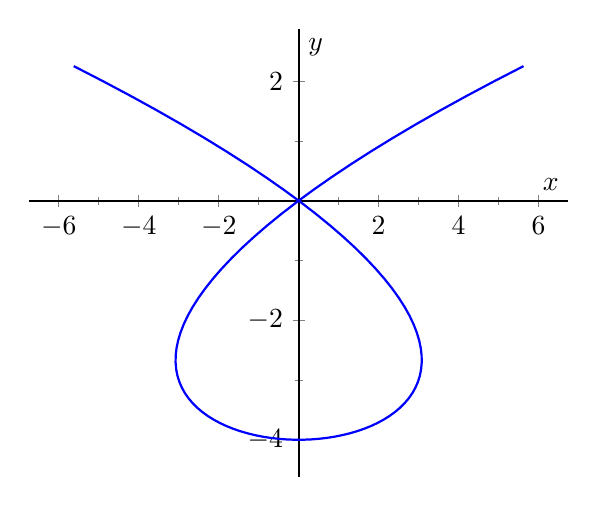
\begin{tikzpicture}
            \begin{axis}[
                % --- CONFIGURACIÓN DE LOS EJES ---
                axis lines = middle,      % Los ejes se cruzan en el (0,0)
                xlabel = {$x$},           % Etiqueta del eje X
                ylabel = {$y$},           % Etiqueta del eje Y
                grid = none,              % Muestra la cuadrícula principal y secundaria
                minor tick num = 1,       % Líneas de cuadrícula intermedias
                enlargelimits = true,     % Añade un pequeño margen a los bordes
                axis line style={-, thick},     % Flechas en los extremos de los ejes
                %
                % Opcional: Esto asegura que si usas sin(t) o cos(t) en el futuro, 
                % LaTeX asuma que 't' está en radianes y no en grados.
                trig format plots=rad,    
            ]
            
            % --- DEFINICIÓN DE LA CURVA PARAMÉTRICA ---
            \addplot [
                domain=-2.5:2.5, % 1. RANGO DE 't': Modifica esto según tu curva
                samples=100,     % 2. SUAVIDAD: Aumenta este número (ej. 200) si la curva tiene picos raros
                variable=\t,     % Definimos que nuestra variable paramétrica es 't'
                thick,           % Grosor de la línea
                blue,            % Color de la línea
            ]
            % 3. ECUACIONES
            % Importante: Usa las llaves { } para agrupar cada componente
            ({t^3 - 4*t}, {t^2 - 4});
            
            \end{axis}
        \end{tikzpicture}
    \end{center}
    Este ejemplo nos permite ver que existen curvas con autointersecciones.
\end{ejemplo}

\begin{ejemplo}
    Consideramos ahora la curva definida como
    \Func{\veps}{I}{\bb{R}^2}{t}{(t^3, t^2)}

    Si estudiamos sus derivadas tenemos
    \begin{gather*}
        \veps'(t) = (3t^2, 2t)\\
        \veps''(t) = (6t,2)
    \end{gather*}
    y obtenemos la siguiente gráfica

    \begin{center}
        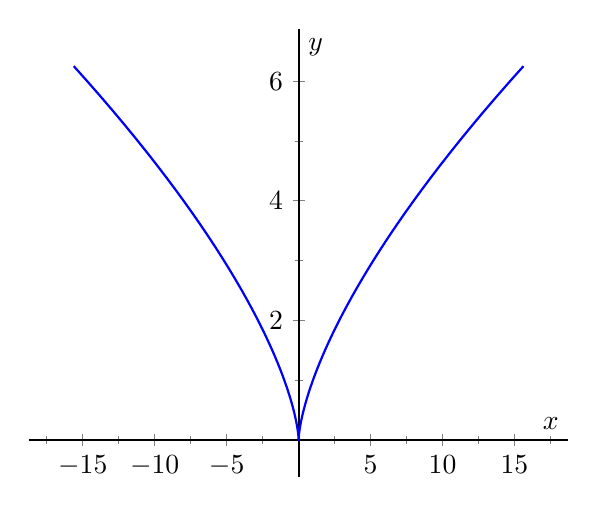
\begin{tikzpicture}
            \begin{axis}[
                % --- CONFIGURACIÓN DE LOS EJES ---
                axis lines = middle,      % Los ejes se cruzan en el (0,0)
                xlabel = {$x$},           % Etiqueta del eje X
                ylabel = {$y$},           % Etiqueta del eje Y
                grid = none,              % Muestra la cuadrícula principal y secundaria
                minor tick num = 1,       % Líneas de cuadrícula intermedias
                enlargelimits = true,     % Añade un pequeño margen a los bordes
                axis line style={-, thick},     % Flechas en los extremos de los ejes
                %
                % Opcional: Esto asegura que si usas sin(t) o cos(t) en el futuro, 
                % LaTeX asuma que 't' está en radianes y no en grados.
                trig format plots=rad,    
            ]
            
            % --- DEFINICIÓN DE LA CURVA PARAMÉTRICA ---
            \addplot [
                domain=-2.5:2.5, % 1. RANGO DE 't': Modifica esto según tu curva
                samples=100,     % 2. SUAVIDAD: Aumenta este número (ej. 200) si la curva tiene picos raros
                variable=\t,     % Definimos que nuestra variable paramétrica es 't'
                thick,           % Grosor de la línea
                blue,            % Color de la línea
            ]
            % 3. ECUACIONES
            % Importante: Usa las llaves { } para agrupar cada componente
            ({t^3}, {t^2});
            
            \end{axis}
        \end{tikzpicture}
    \end{center}

    Este ejemplo nos demuestra que aunque $\veps$ sea diferenciable, $tr(\veps)$ tiene ``picos''. Tenemos que $img(\veps) = Gr\{y=x^{\nicefrac{2}{3}}\}$, es decir, la traza de $\veps$ coincide con la gráfica de una función no diferenciable.
\end{ejemplo}

\begin{ejemplo} Consideramos la siguiente curva
    \Func{\zeta}{\bb{R}}{\bb{R}^3}{t}{a+r(e_1\cos(\frac{t}{r}) + e_2(\sen(\frac{t}{r})))}
    donde $r>0$, $a\in \bb{R}^3$, $e_1,e_2\in \bb{R}^3$ tal que $|e_1|=|e_2|=1$ y $\langle e_1,e_2 \rangle = 0$.

    Como tenemos 2 vectores ortogonales en el espacio, estos generarán un plano, por lo que $\zeta(t)\in P = a + \langle \{e_1,e_2\}\rangle$ $\forall t \in \bb{R}$. Por tanto
    \begin{gather*}
        img(\zeta) = tr(\zeta) \subset P \Rightarrow \zeta \text{ es una curva plana}
    \end{gather*}
    Además, se verifica que 
    \begin{gather*}
        |\zeta(t) - a | = r \ \ \forall t\in \bb{R}
    \end{gather*}
    lo que nos dice que todos los puntos de la traza equidistan al punto $a$, llegando a la conclusión de que $tr(\zeta)$ es una circunferencia centrada en $a$. A esta curva la llamaremos \underline{la} circunferencia de centro $a$ y radio $r>0$ en $P$.\\

    Podemos ver también que esta curva no se recorre de una forma aleatoria:
    \begin{gather*}
        \zeta'(t) = -e_1\left(\sen\left(\frac{t}{r}\right)\right) + e_2\left(\cos\left(\frac{t}{r}\right)\right) \Rightarrow \text{ no es un MRU}\\
        \zeta''(t) \text{ no es constante} \Rightarrow \text{ no es un movimiento rectilíneo acelerado}
    \end{gather*}
    Si estudiamos un poco más esta curva veremos que la aceleración es solo centrífuga ya que $|\zeta''(t)|=1$. Esta es la traza de un MCU\footnote{Movimiento Circular Uniforme}.
\end{ejemplo}

\begin{ejemplo}
    Definimos la siguiente curva
    \Func{\eta}{I}{\bb{R}^2}{t}{\left(\frac{3t}{1+t^3}, \frac{3t^2}{1+t^3} \right)}
    donde $I=]-1, +\infty[$. La gráfica será algo como\footnote{a esta curva se le conoce como Hoja de Descartes}

    \begin{center}
        \begin{tikzpicture}
            \begin{axis}[
                % --- CONFIGURACIÓN DE LOS EJES ---
                axis lines = middle,      % Los ejes se cruzan en el (0,0)
                xlabel = {$x$},           % Etiqueta del eje X
                ylabel = {$y$},           % Etiqueta del eje Y
                grid = none,              % Muestra la cuadrícula principal y secundaria
                minor tick num = 1,       % Líneas de cuadrícula intermedias
                enlargelimits = true,     % Añade un pequeño margen a los bordes
                axis line style={-, thick},     % Flechas en los extremos de los ejes
                %
                % Opcional: Esto asegura que si usas sin(t) o cos(t) en el futuro, 
                % LaTeX asuma que 't' está en radianes y no en grados.
                trig format plots=rad,    
            ]
            
            % --- DEFINICIÓN DE LA CURVA PARAMÉTRICA ---
            \addplot [
                domain=-0.85:50, % 1. RANGO DE 't'
                samples=500,     % 2. SUAVIDAD: Aumenta este número (ej. 200) si la curva tiene picos raros
                variable=\t,     % Definimos que nuestra variable paramétrica es 't'
                thick,           % Grosor de la línea
                blue,            % Color de la línea
            ]
            % 3. ECUACIONES
            % Importante: Usa las llaves { } para agrupar cada componente
            ({(3*t)/(1+t^3)}, {(3*t^2)/(1+t^3)});
            
            \end{axis}
        \end{tikzpicture}
    \end{center}

    Tendremos que ver que $\eta$ es inyectiva (o lo que es lo mismo, no tiene autointersecciones). Observamos también que $\eta'(t)\neq 0$ $\forall t \in I$. Nos preguntamos si $I\cong tr(\eta)$ es un homeomorfismo y llegamos a la conclusión de que no lo es (si quitamos el punto $(0,0)$ en la $tr(\zeta)$ obtenemos una única componente conexa, ya que $\overline{(tr(\zeta)\setminus\{(0,0)\})} = tr(\zeta)$, pero al quitar cualquier punto en $I$ obtendremos dos componentes).
\end{ejemplo}

\begin{definicion}
    Sea $I\subset \bb{R}$ un intervalo, $\alpha: I \to \bb{R}^3$ una curva, definimos la recta tangente a $\alpha$ en el instante $t\in I$ como la recta afín $\alpha(t) + \langle \alpha'(t) \rangle$ y la representamos como $R_{\alpha(t), \alpha'(t)}\equiv R_t$.
\end{definicion}

\begin{observacion}
    Si $\alpha'(t)=0$, entonces la recta tangente será $\alpha(t) + \langle 0 \rangle = \alpha(t)$ que no será una recta, sino un punto. Por tanto, en los puntos $t\in I$ con $\alpha'(t)=0$ no existirá recta tangente. Esto nos dará motivos para intentar evitar esta situación.
\end{observacion}

\begin{definicion}
    Sea $I\subset \bb{R}$ un intervalo, $\alpha: I \to \bb{R}^3$ una curva. Los puntos $\alpha(t)\in tr(\alpha)$ tales que $\alpha'(t)\neq 0$ se llaman \textbf{regulares}. A los puntos que no verifican esta condición los llamaremos \textbf{singulares}.\\

    La curva $\alpha$ se dice \textbf{regular} si $\alpha'(t)\neq 0$ $\forall t \in I$, es decir, si todos los puntos $t\in I$ son regulares.
\end{definicion}



